\documentclass[utf8]{ctexart}


\usepackage{amssymb}
\usepackage{enumerate}
\usepackage[numbers]{natbib} 
\usepackage{geometry}
\usepackage{wrapfig}
\geometry{left=3.0cm,right=3.0cm,top=2.5cm,bottom=2.5cm}
\usepackage{fancyhdr}
\pagestyle{fancy}
\lhead{}
\rhead{}
	\setlength{\headheight}{10mm}
   \fancyhead[C]{
   	\begingroup
   	\setlength{\tabcolsep}{10pt} % Default value: 6pt
   	\renewcommand{\arraystretch}{1.5} % Default value: 1
\begin{tabular}{ccc}
         & \large{\textbf{卢瑟福散射实验报告}} &  \\
     少年班学院 \qquad \qquad & PB20000069 刘子安 & \qquad \today
\end{tabular}
\endgroup
}
\fancyfoot[C]{ 第 {\thepage} 页,共 \pageref{unknown} 页}
\renewcommand{\headrulewidth}{0pt}
 

\usepackage{graphicx}



\begin{document}

\section*{实验目的}
\begin{enumerate}
	\item 
	复习用卢瑟福散射公式,推导$\alpha$粒子散射公式
	\item 
	了解卢瑟福散射谱仪的结构和工作原理
	\item 
	用实验验证卢瑟福散射公式
\end{enumerate}



\section*{实验原理}
\subsection*{实验仪器:} 
\par
尺子、空靶、金靶、真空泵、散射室、步进电机及其控制系统、数据采集系统和电脑多道软件。
\subsection*{实验原理\cite{bk1}:}
\begin{wrapfigure}{r}{6cm}
	\centering
	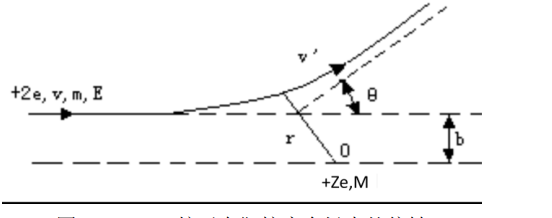
\includegraphics[scale=0.7]{1.1.png}
	\caption{$\alpha$粒子在靶核库仑场中的偏转}
\end{wrapfigure}
(1)库仑散射公式的完整推导:
\par
设原子核的质量为$M$,具有正电荷$+Ze$,并且位于原点$O$处,质量为$m$,能量为$E$,电荷为$2e$的$\alpha$粒子以速度$v$入射,在原子核(靶核)的质量比$\alpha$粒子的质量大得多的情况下,可以认为前者不被推动,$\alpha$粒子则受到库仑力的作用而改变了运动的方向,偏转$\theta$角。如图1所示。图中$b$是原子核离$\alpha$粒子原运动路径延长线的垂直距离,即入射原子与原子核无作用时的最小直线距离,称为瞄准距离。

由能量和动量守恒定律,有:
\begin{equation}
	E = \frac{1}{4\pi\varepsilon_0}\frac{2Ze^2}{r}+\frac{m}{2}(\dot{r}^2+r^2\dot\varphi^2)
\end{equation}
\begin{equation}
	L = mr^2\dot\varphi = m \dot{v}b
\end{equation}

由(2)式可得$\dot{\varphi} = L/mr^2$并且有$\dot{r} = \frac{dr}{dt} =  \frac{dr}{d\varphi}\dot{\varphi}$,将其代入(1)式并两边同乘$\frac{m^2}{L^2}$可得:
\begin{equation}
	\frac{2mE}{L^2}=\frac{1}{r^4}(\frac{dr}{d\varphi}) + \frac{1}{r^2} + \frac{4Ze^2m}{4\pi\varepsilon_0L^2}\frac{1}{r}
\end{equation}

我们令$\rho = \frac{1}{r}$,则$\frac{dr}{d\rho} = -\frac{1}{\rho^2}$将其代入(3)式并化简,有:
\begin{equation}
	\frac{2mE}{L^2} = -2C\rho+\left(\frac{d\rho}{d\varphi}\right)^2+\rho^2
\end{equation}

其中$C = -\frac{2Ze^2m}{4\pi\varepsilon_0L^2}$,我们再把等式的两边对$\varphi$求导并同时除以$2\frac{d\rho}{d\varphi}$可以得到:
\begin{equation}
	\frac{d^2\rho}{d\varphi^2}+\rho = C
\end{equation}

可以得到方程的解为:
\begin{equation}
	\rho = A\cos{\varphi} + B\sin{\varphi} + C
\end{equation}

其中$A,B$为常数,代入初始条件$\varphi \to \pi$时,有$\rho = \frac{1}{r} \to 0$ 并且 $r\sin{\varphi} = b$可以定出:
\begin{equation}
	\rho = \frac{1}{r} = C(1+\cos{\varphi} + \frac{1}{b}\sin{\varphi})
\end{equation}

当$\alpha$粒子以$\theta$角被散射到无穷远时,即此时有$\varphi \to \alpha$,$\rho \to 0$,再令$a = \frac{2Ze^2}{4\pi\varepsilon_0E}$消去$C$可得:
\begin{equation}
	ctg\frac{\theta}{2} = -\frac{1}{Cb} = \frac{2b}{a}
\end{equation}

此即为库仑散射公式。

\begin{wrapfigure}{r}{8cm}
	\centering
	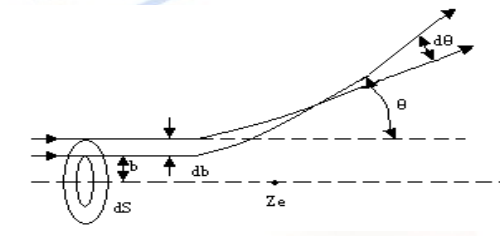
\includegraphics[scale=0.8]{1.2.png}
	\caption{$\alpha$粒子散射角与瞄准距离的关系}
\end{wrapfigure}
(2)卢瑟福散射公式的完整推导
\par
库仑散射定律中的瞄准距离$b$是实验中无法测量的,我们想办法去找一个实验中可以测量的量。
事实上,虽然单个$\alpha$粒子的瞄准距离$b$我们无法测量,但是大量$\alpha$粒子的散射具有一定的统计规律。那些瞄准距离在$b\sim b+db$之间的$\alpha$粒子,经散射后必定从$\theta \sim \theta - d\theta$的角度出射。
\par 
设靶是一个很薄的箔,厚度为$t$,面积为$s$,则图2中的$ds = 2\pi b|db|$,一个$\alpha$粒子靶原子散射到环$dS$上的概率。利用式(8)可得:
\begin{equation}
	\frac{dS}{S} = \frac{2\pi b|db|}{S} = \frac{\pi a^2\cos{\frac{\theta}{2}}}{4S\sin^3{\frac{\theta}{2}}}
\end{equation}
又由于立体角:
$$
d\Omega = 2\pi \sin{\theta} = 4\pi \sin{\frac{\theta}{2}}\cos{\frac{\theta}{2}}d\theta
$$

为了求得为求得实际的散射$\alpha$粒子数,以便与实验进行比较,还必须考虑靶上的原子数和入射的$\alpha$粒子数。由于薄箔有许多原子核,每一个原子核对应一个这样的环,若各个原子核互不遮挡,设单位体积内原子数为$n$,则体积$St$内原子数为$nSt$,$\alpha$粒子打在这些环上的散射角均为$\theta$,因此一个$\alpha$粒子打在薄箔上,散射到$\theta$方向且在$d\Omega$内的概率为$\frac{dS}{S}nts$

若单位时间内有$N$个$\alpha$粒子垂直入射到薄箔上,则单位时间内$\theta$方向且在$d\Omega$立体角内测得的$\alpha$粒子为:
\begin{equation}
	dn = N\frac{dS}{S}nts = \left(\frac{1}{4\pi \varepsilon_0}\right)^2nNt\left(\frac{2Ze^2}{4E}\right)^2\frac{d\Omega}{\sin^4{\frac{\theta}{2}}}
\end{equation}

常用的是微分散射截面的公式:
\begin{equation}
	\frac{dS}{d\Omega} = \frac{a^2}{16\sin^4{\frac{\theta}{2}}} = \left(\frac{1}{4\pi \varepsilon_0}\right)^2\left(\frac{Ze^2}{2E}\right)^2\frac{1}{\sin^4{\frac{\theta}{2}}}
\end{equation}

此即著名的卢瑟福散射公式。


\section*{实验记录及数据处理}
\subsection*{实验数据:}

我们在使用空靶时对物理$0^{\circ}$角在不同气压下测量它的ROI计数,每次测量均为$120s$:
\begin{table}[!ht]
	\centering
	\caption{测得气压P与选区计数N的关系}
\begin{tabular}{|c|c|c|c|c|c|c|}
	\hline
	$P/kPa$ & 0.0 & 6.0 & 12.0 & 18.0 &  24.0 & 30.2 \\
	\hline
	选区计数N & 260172 & 223659 & 194049 & 160276 & 120132 & 77662 \\
	\hline
\end{tabular}
\end{table}

我们再使用金靶,并对$10^{\circ}$到$22^{\circ}$之间几个角度进行了不同时间的测量:
\begin{table}[!ht]
	\centering
	\caption{测得不同角度对应时间下的选区计数N}
	\begin{tabular}{|c|c|c|c|c|c|}
		\hline
		角度$^{\circ}$ & 10 & 13 & 16 & 19 & 22 \\
		\hline
		$\frac{1}{\sin^4{\theta/2}}$ & 17330 & 6089 & 2666 & 1348 & 754 \\
		\hline
		时间t$/s$ & 200 & 300 & 600 & 900 & 1200 \\
		\hline
		计数$N$ & 5891 & 4286 & 3712 & 2602 & 1707 \\
		\hline
		每秒选区计数$\frac{N}{t}/s^{-1}$ & 29.46 & 14.29 & 6.19 & 2.89 & 1.42 \\
		\hline
	\end{tabular}
\end{table}

\subsection*{数据处理:}
绘制空靶时的$N-P$图:
\begin{figure}[htbp]
	\centering
	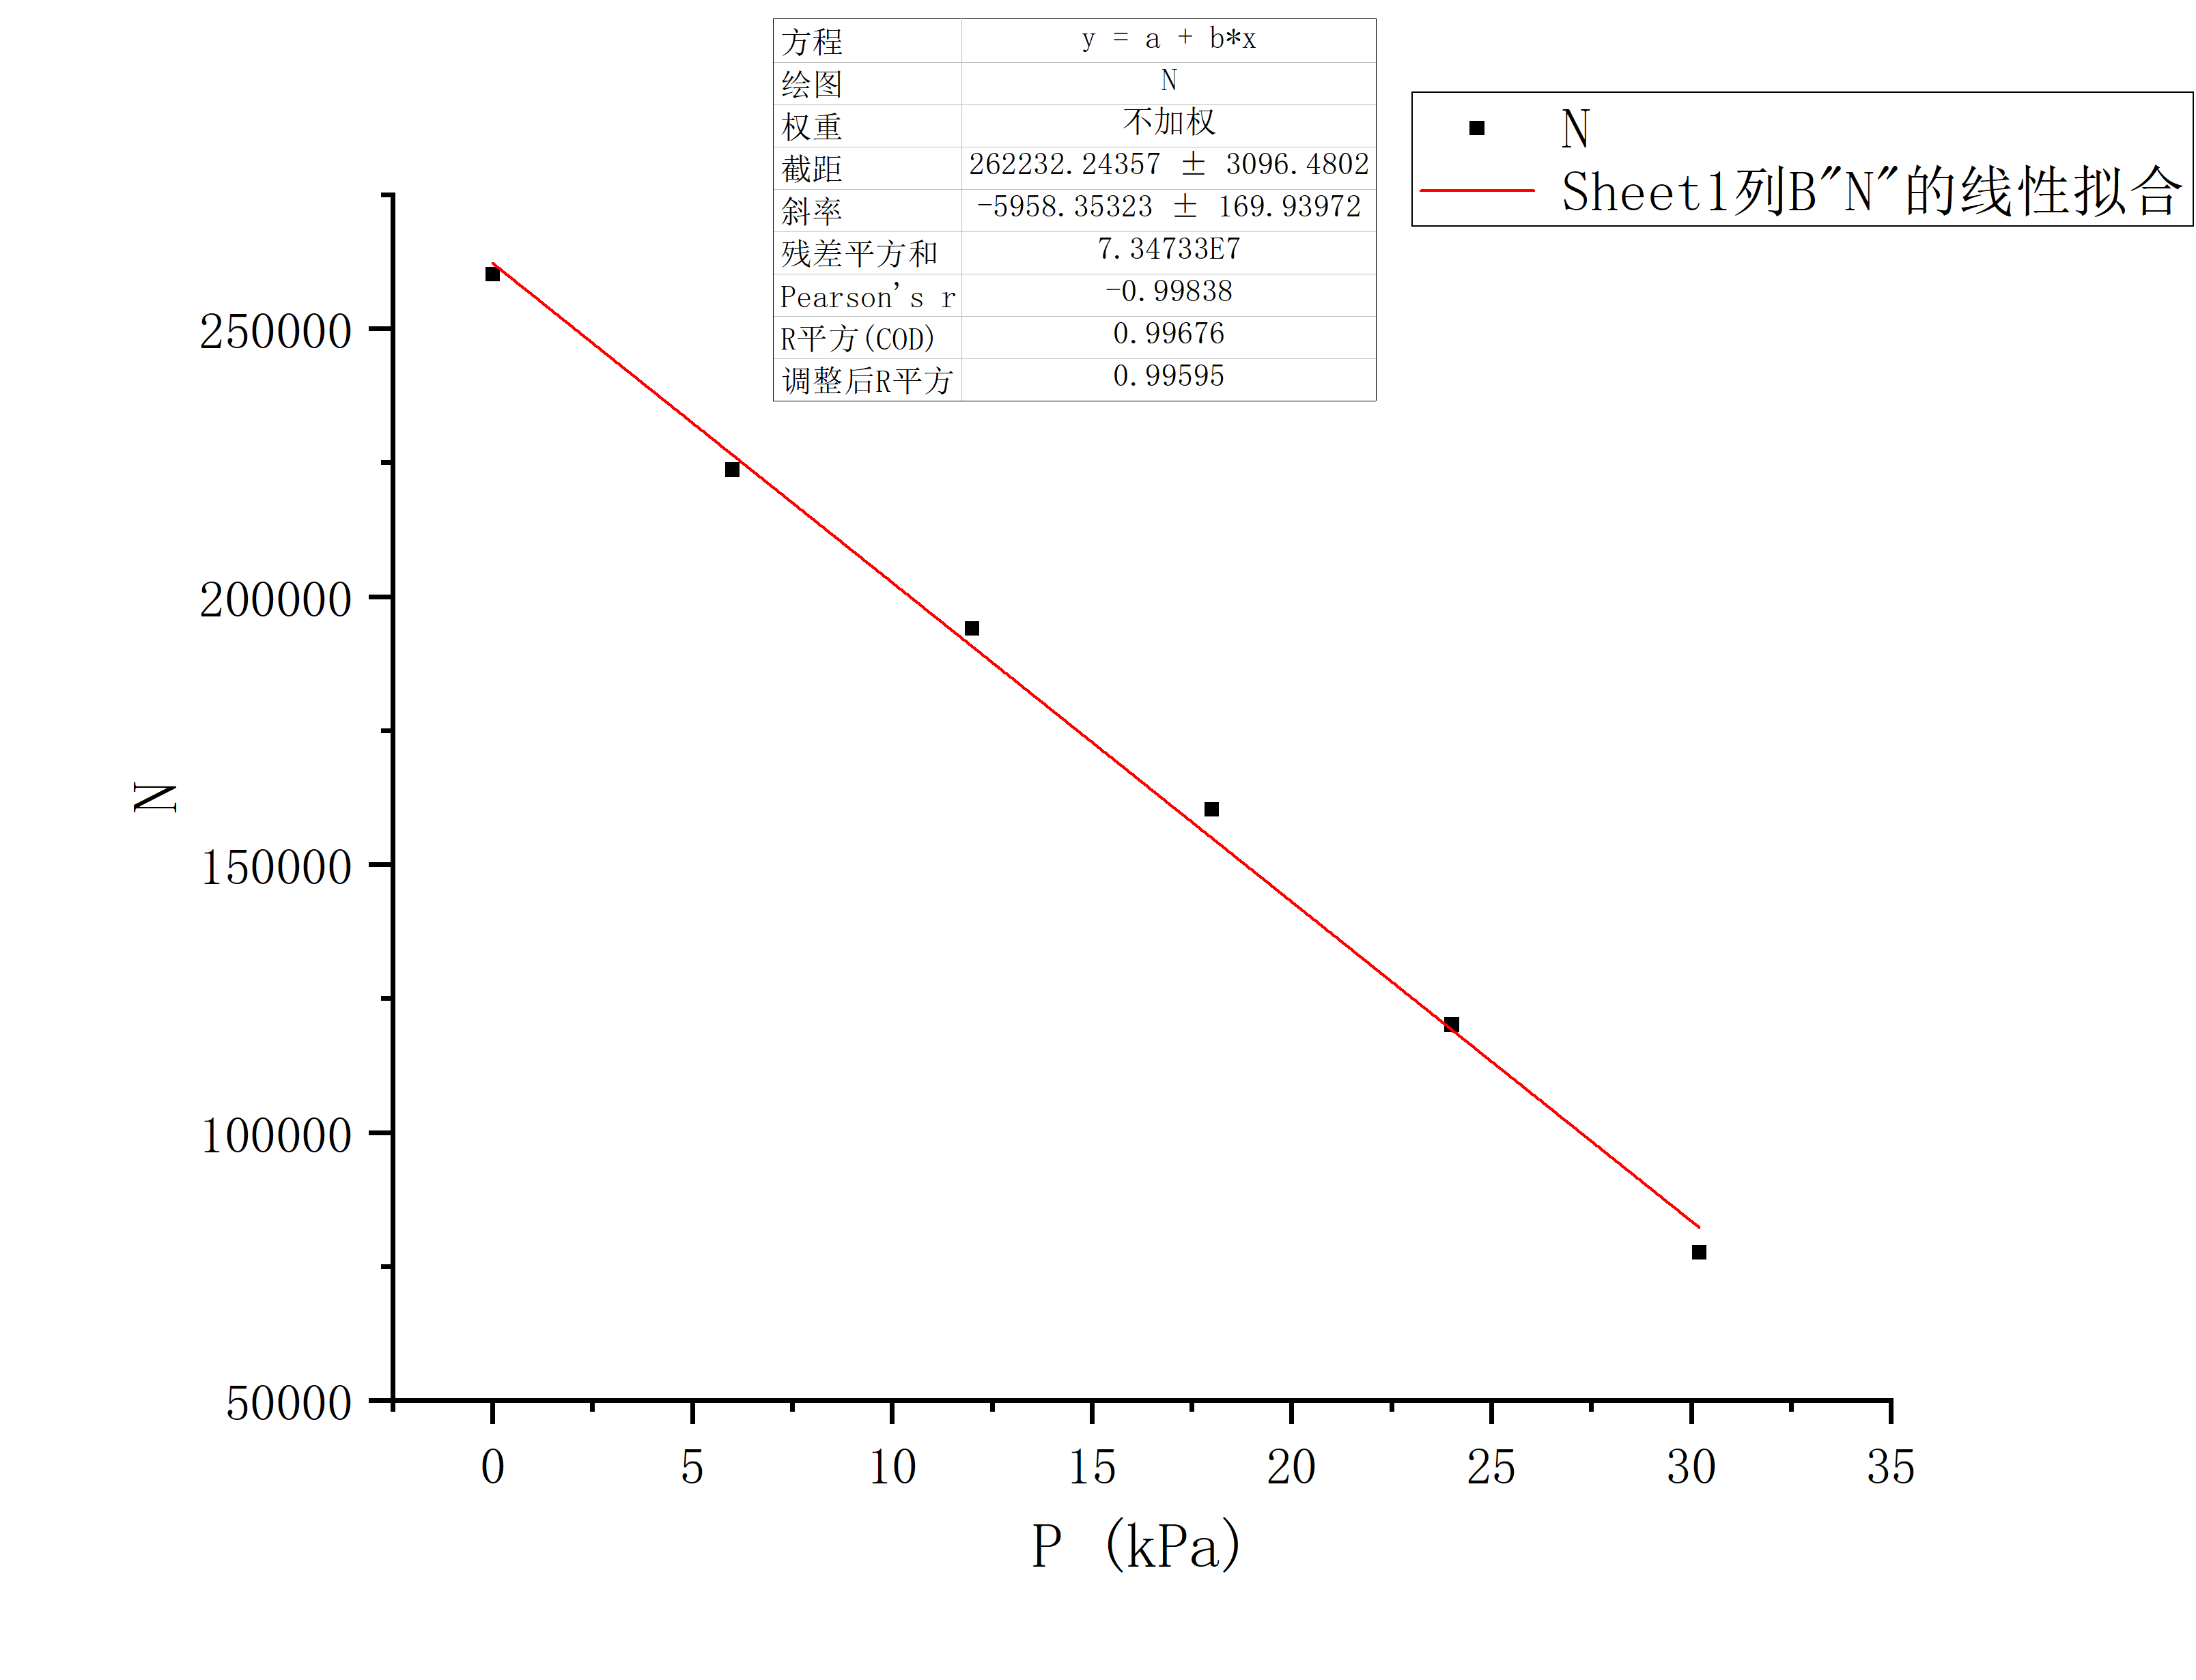
\includegraphics[scale=0.4]{Graph1.png}
	\caption{空靶时的$N-P$图}
\end{figure}

我们可以得到$N_0 = 262232$,从图中还可以知道:
\begin{equation}
	N = a+bP = 262232 - 5958P
\end{equation}

上式中$P$的单位为$kPa$,此时温度为:
$$
T = \frac{T_1+T_2}{2} = \frac{24.4+25.5}{2} = 24.95^{\circ}C = 298.1 \; K
$$

$N=N_0/2 = 131116$时有:
$$
P = 22.0\;kPa
$$

此时$\alpha$粒子的平均射程为$l_2 = 73.0 \; mm$。

再使用附录$2$中的公式,求出此时的空气密度:
\begin{equation}
	\rho_1 = 1.293 \times \frac{22.0}{101.325} \times \frac{273}{298.1} = 0.257 \; kg/m^3
\end{equation}

代入密度与射程的关系$\rho_0 R = \rho_1 l_2 $可以得到在标准大气压下的平均射程为:
\begin{equation}
	R = \frac{\rho_1}{\rho_0}l_2 = \frac{0.257}{1.293}7.30 \; cm = 1.45 \; cm
\end{equation}

由经验公式$R = (0.285 + 0.005E)E^{1.5}$ ,使用Origin绘制$E$从$0$到$10$的函数图像,并取其与$R=1.45$的交点:
\begin{figure}[htbp]
	\centering
	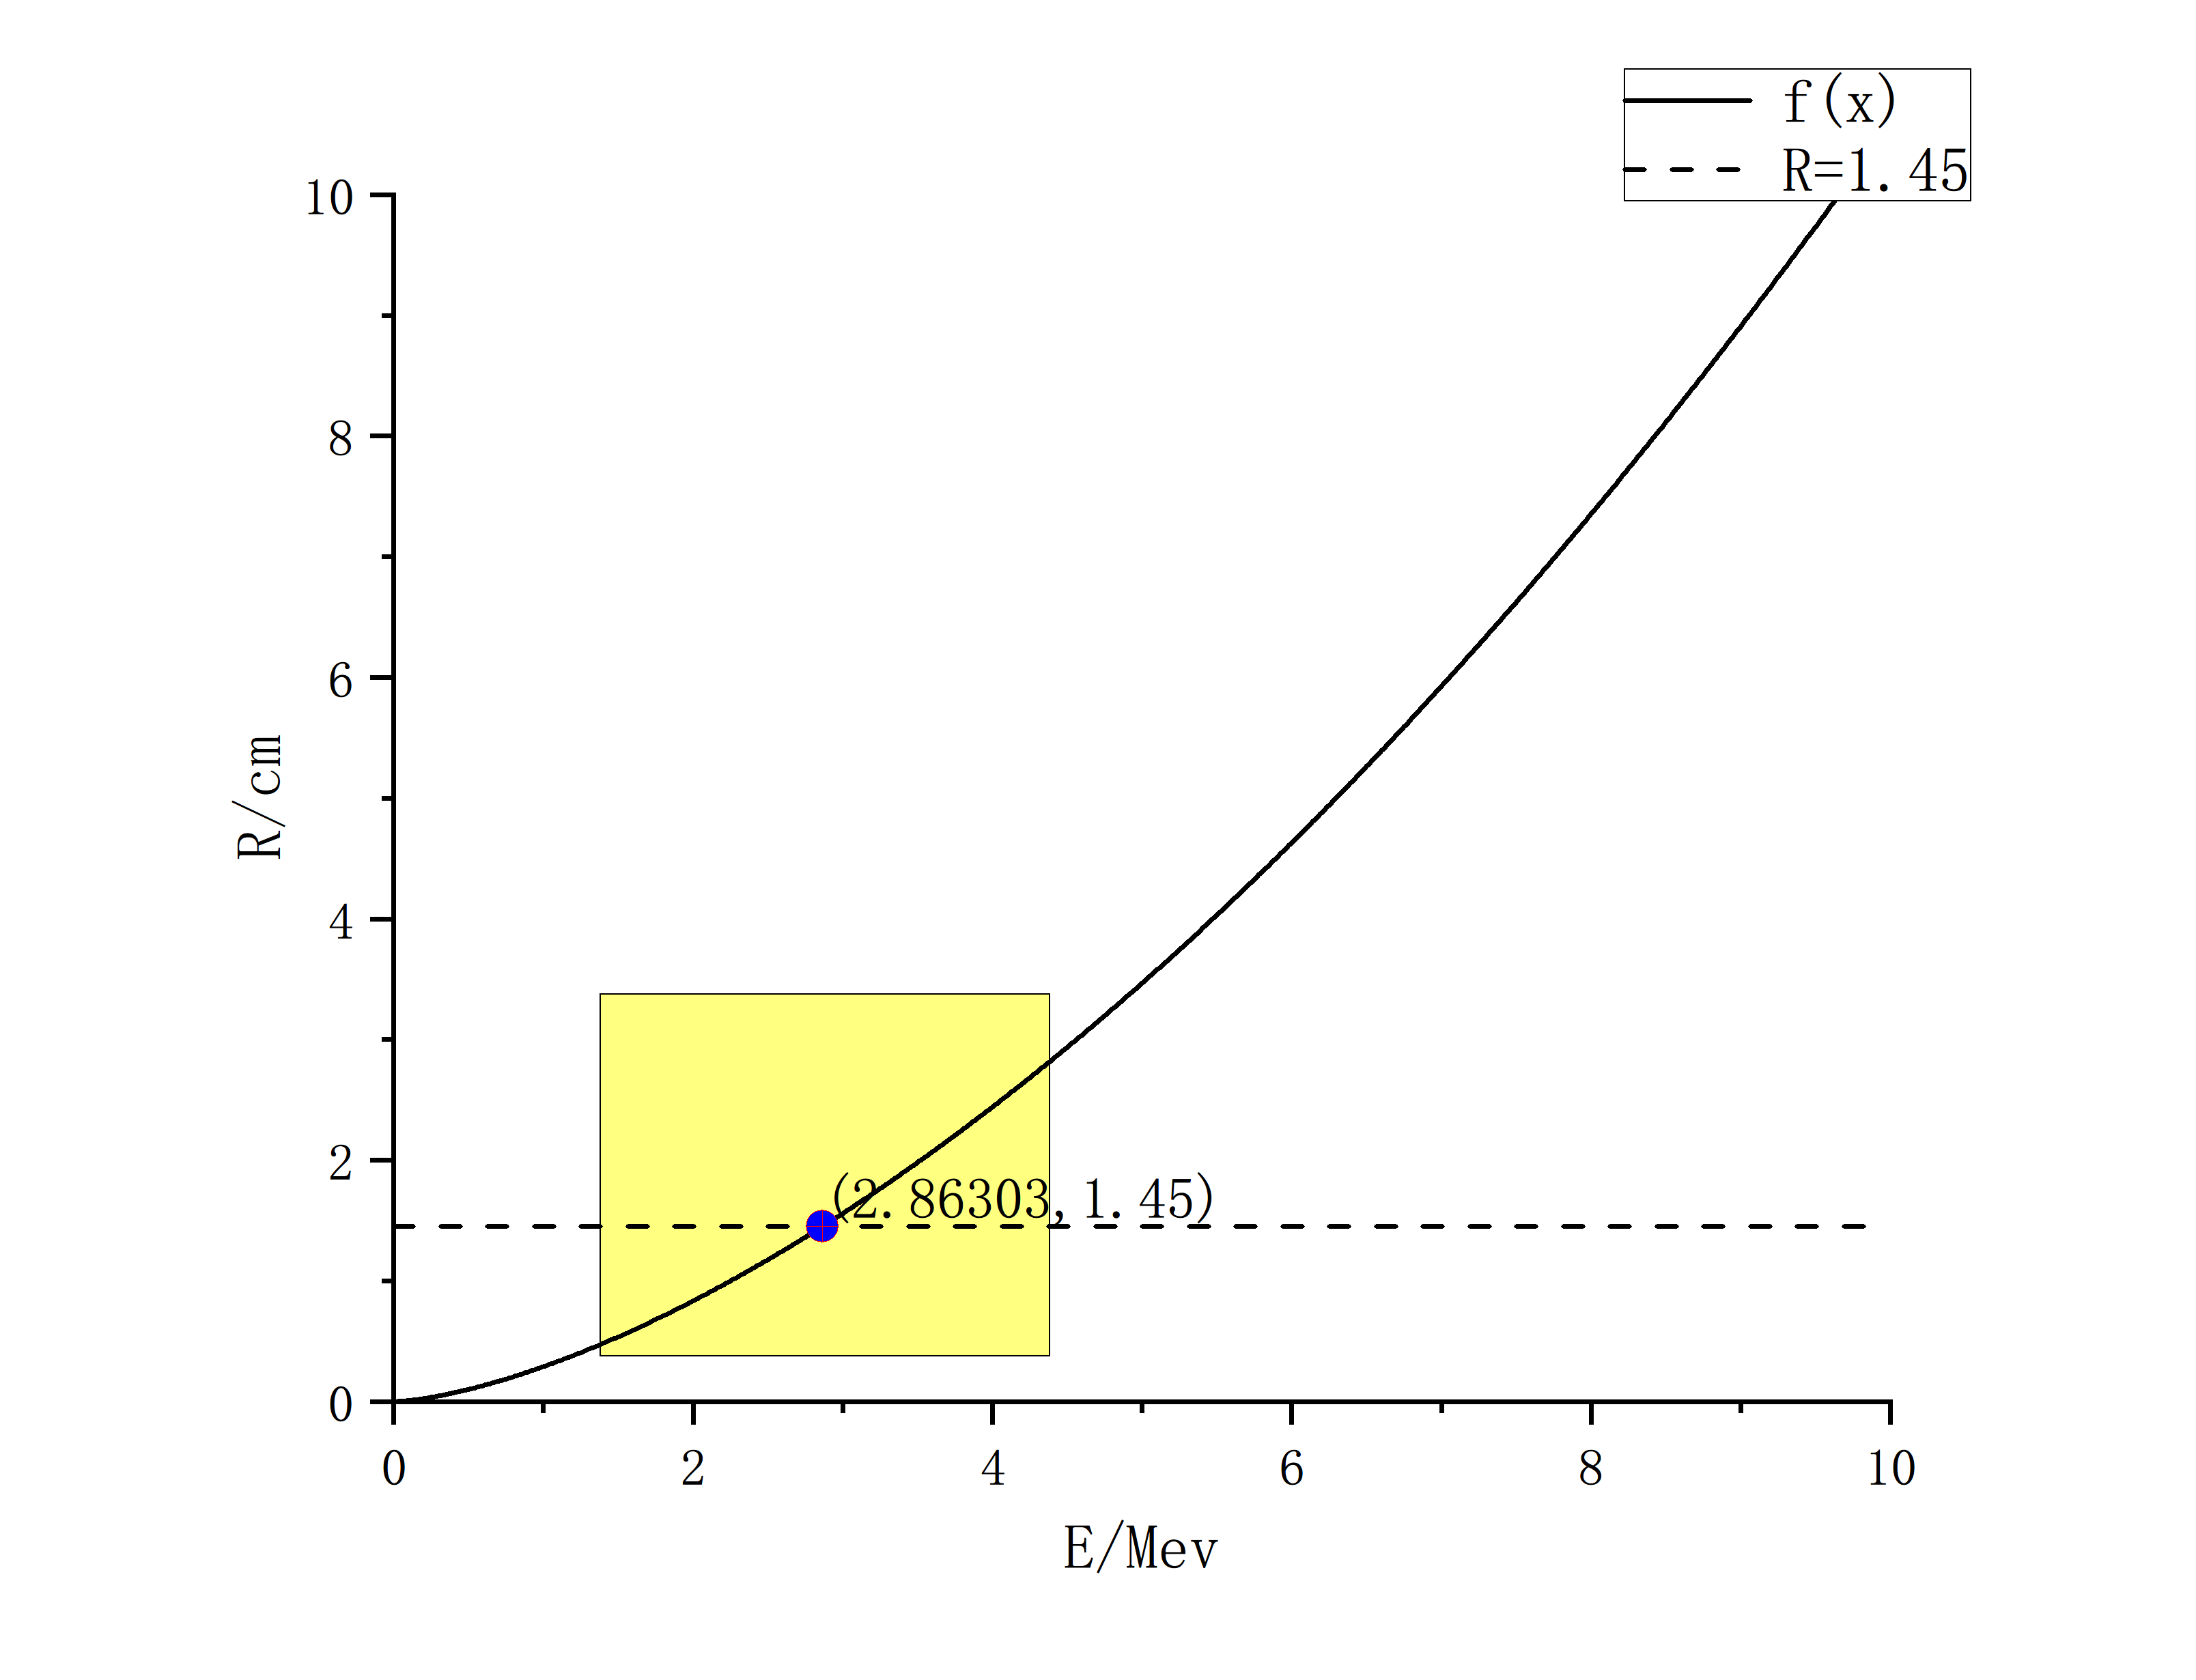
\includegraphics[scale=0.4]{Graph2.png}
	\caption{$R$与$E$的关系图}
\end{figure}
从图中我们可以得到,从源出射的$\alpha$粒子的能量:
\begin{equation}
	E = 2.86 MeV
\end{equation}
与实际的能量(约为$5MeV$)相差较大,我认为这主要是由于气压的测量误差较大造成的,也可能受到了系统误差的影响而导致计数不够准确。
\\
接下来我们换上金靶,并且抽真空后测量,调整到物理零度角。绘制$N-\frac{1}{\sin^4{\theta/2}}$图:
\begin{figure}[!htbp]
	\centering
	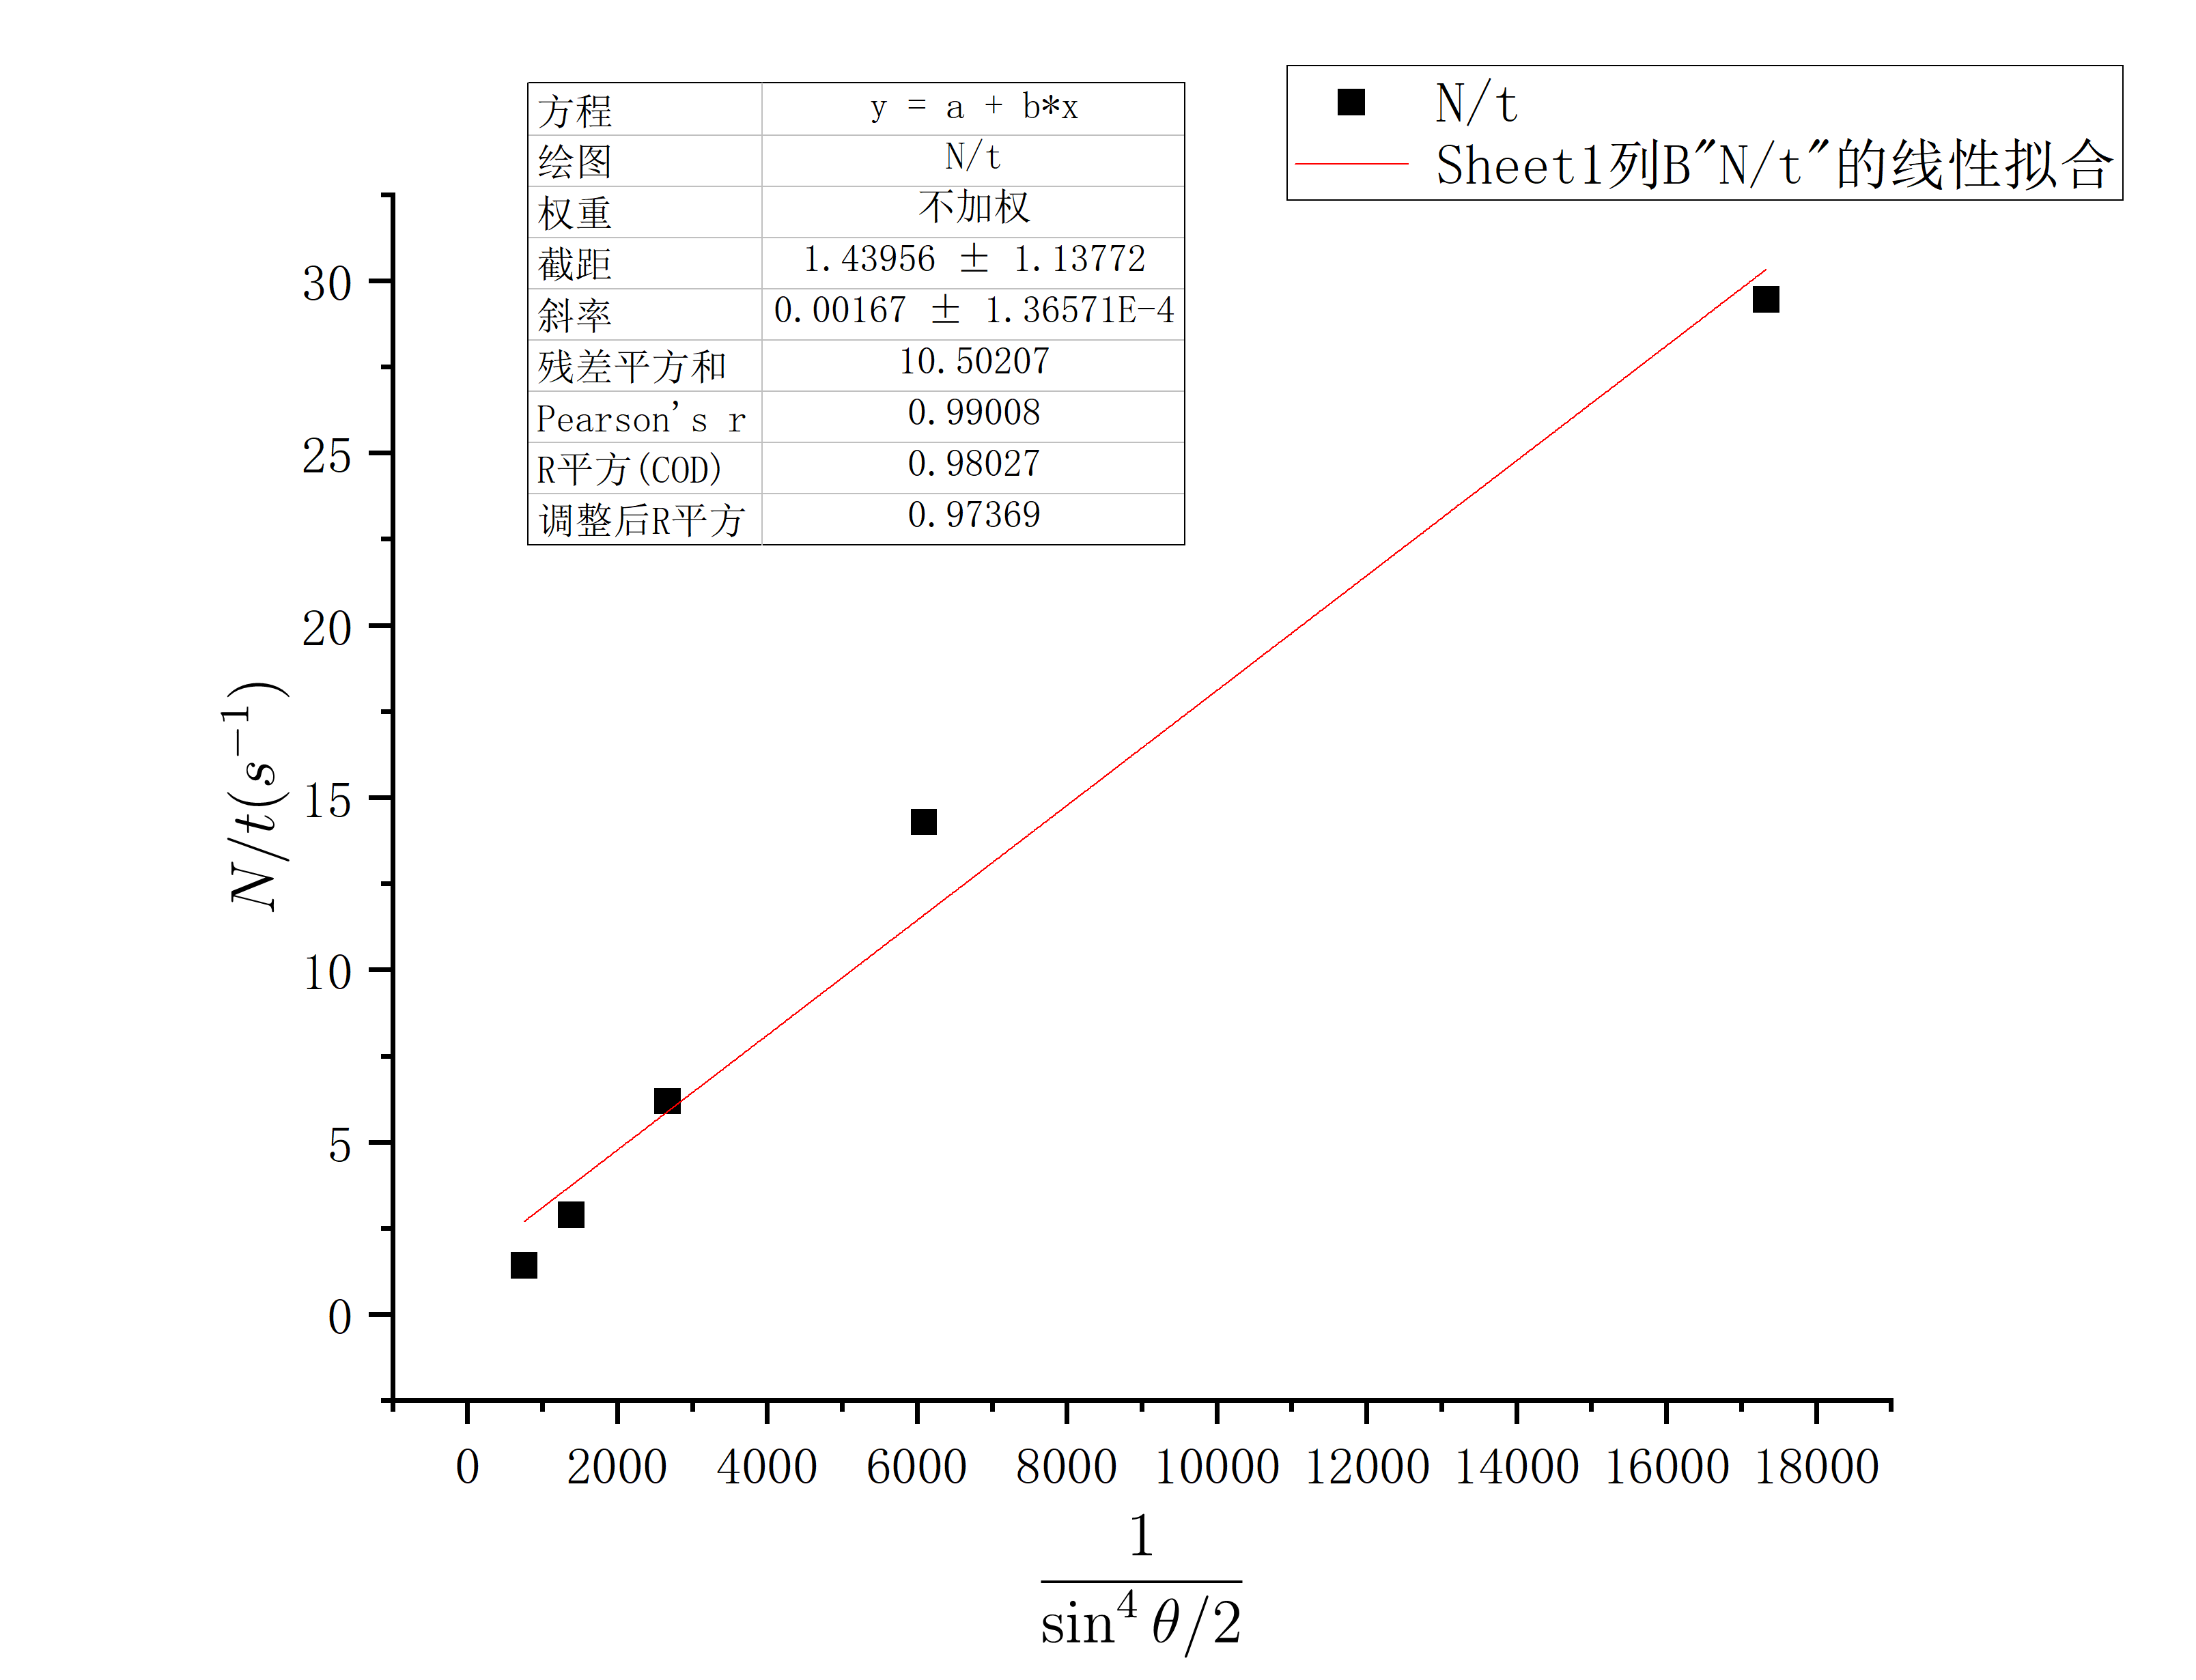
\includegraphics[scale=0.35]{Graph3.png}
	\caption{$N-\frac{1}{\sin^4{\theta/2}}$图}
\end{figure}

从图中可以看到线性拟合的$r^2=0.99$,线性拟合度比较好,可以近似认为$K=N\sin^4{\theta/2}$为一常数,$K$的实验值为:
\begin{equation}
	K = 1.67 \times 10^{-3} \; s^{-1}
\end{equation}

再计算$K$的理论值为:
\begin{equation}
	K=4.8065 \times 10^{-34}\frac{N_0}{E^2l_1^2} = 4.8065 \times 10^{-34}\frac{262232}{(2.86 \times 10^6 \times 1.6\times{10^{-19}})^2 \times 0.44^2} = 3.11 \times 10^{-3} \; s^{-1}
\end{equation}

两者比较接近。接下来绘制$K-\theta$曲线图:
\begin{figure}[!htbp]
	\centering
	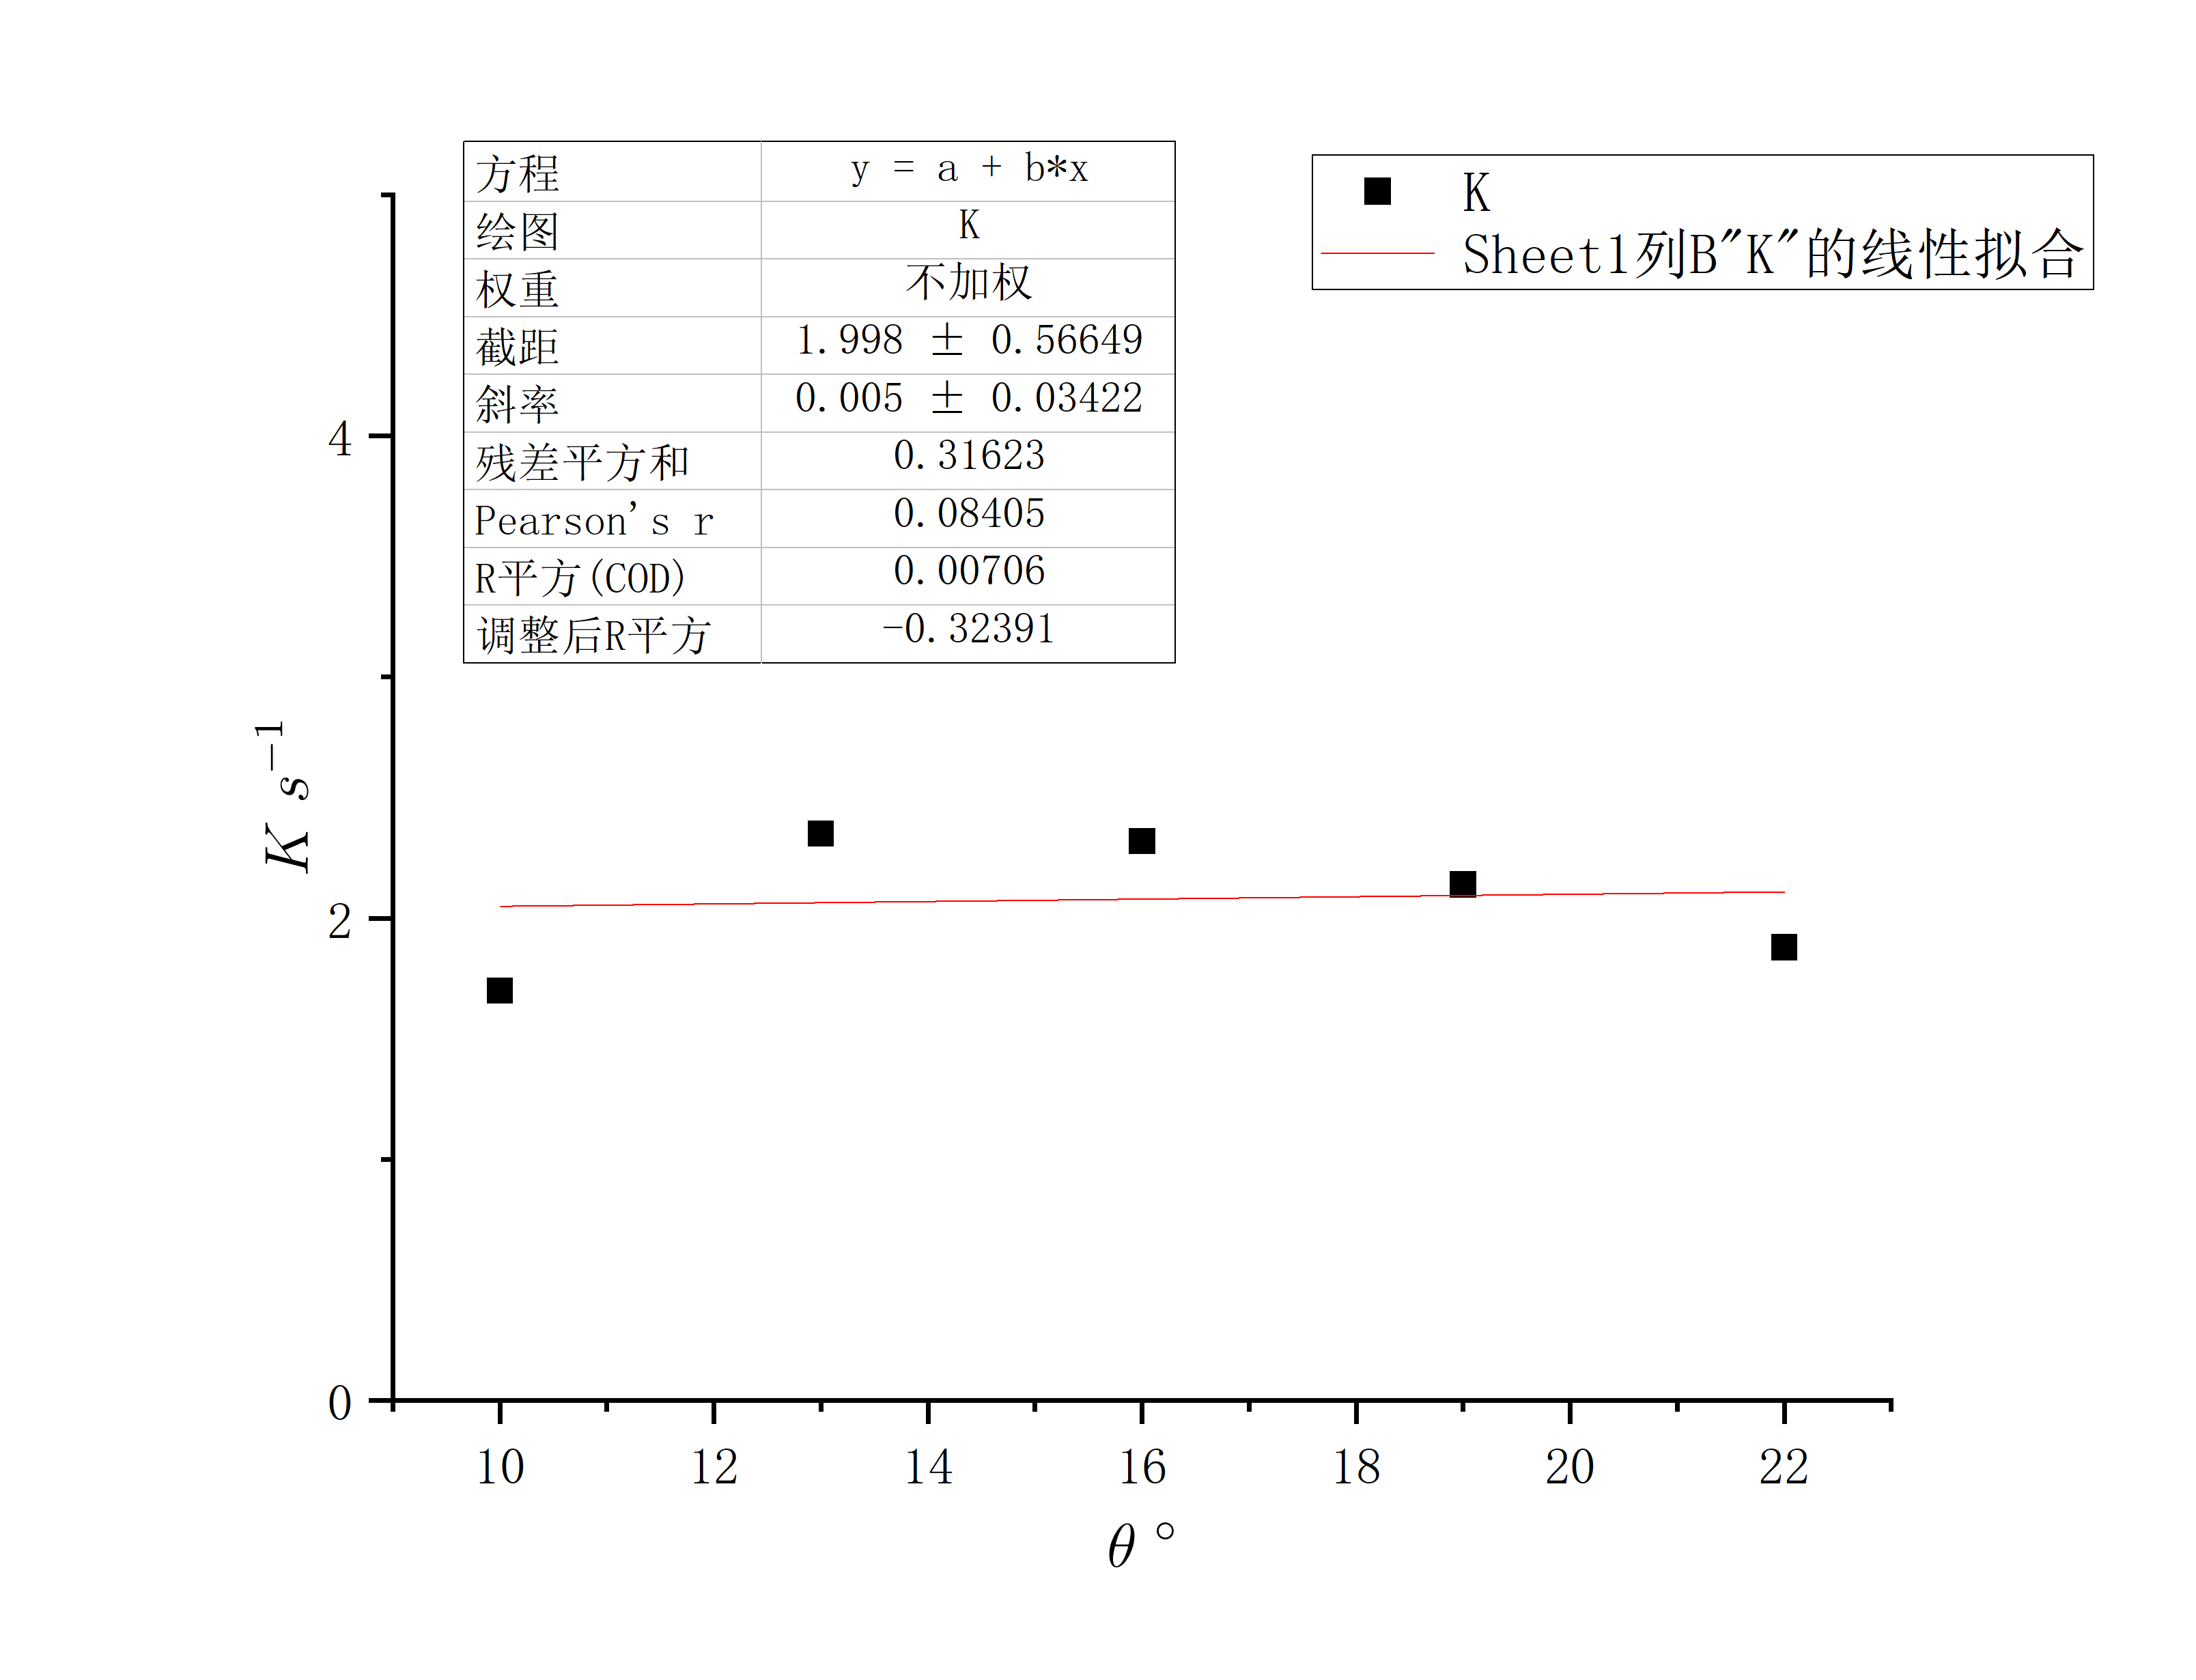
\includegraphics[scale=0.37]{Graph4.png}
	\caption{$K-\theta$图}
\end{figure}

从图中我们可以发现,$K$随$\theta$的变化还是比较大的,也就是说实验结果与卢瑟福散射得到的$K$应为常数有一定偏差。具体原因写在思考题中。


\section*{思考题}

\begin{itemize}
   \item [2.] 根据卢瑟福公式$N\sin^4{\frac{\theta}{2}}$应该为常数,本实验的结果有偏差吗?试分析原因。
   \item [ ] 答: 实验结果有一定偏差,原因如下:
   \begin{itemize}
   	\item 实验所测试的角度都比较小,在观察较小的$\theta$角的散射时,实际上它是由多次小角散射合成的。既然都是小角散射,那每一个都不能忽略,从而一次散射理论不再适用\cite{bk2}。
   	\item 另外,在$\theta$很小时,相当于瞄准距离$b$很大,从而应该需要考虑原子核外电子的屏蔽效应和原子核有限质量对散射截面的影响\cite{art1}。但是从参考文献\cite{art1}中也可以发现,与结果仍有出入。
   	\item 实验中$\alpha$粒子有一定展宽\cite{art2}、在不同散射核处,大小相同的各有效截面对应的$d\Omega$是不一样的,卢瑟福散射公式的推导过程中忽略了这一点。
   	\item 实验中的系统误差,从而使得我们的测量不够准确,比如计数不够准确、真空并非“真空”。
   	\item 测量误差,对长度的测量不够准确,还有在确定物理0度时也有一定偏差,在测量时未考虑转动的回程差等。
   	\item 环境造成的误差,手机等产生的电磁波会导致带电粒子的偏转。
   \end{itemize}
   \item [3.] 若人体肌肉组织的密度为 $1.10g/cm3$,根据实验内容4的结果估算本实验中的$\alpha$粒子在
   人体肌肉组织中的射程,单位取 $cm$。
   \item [ ] 答: 代入公式$\rho R = Const$可得 $R = \frac{\rho_1}{\rho}l_2 = 
   \frac{0.257}{1100} \times 7.30 \; cm = 1.71 \times 10^{-3} \; cm $
\end{itemize}

\section*{总结}
本次实验总体完成的比较成功,但是在做完实验后也出现了一些疑问,有些查阅了资料后有了一些了解,但是仍然没有完全解决:
\begin{itemize}
	\item 在空靶时的$\alpha$粒子散射实验中,随着压强$P$的增大,选区计数的数目也在不断下降,并且基本是线性关系。但是如果根据卢瑟福散射定律,等效厚度$t$的增大应该导致$N$的线性增大,但是由于此时的$\theta$角很小,应该并不满足卢瑟福散射定律,那么如何解释这个现象?在网上查询一些资料后发现$\alpha$粒子在空气中接近射程时会被吸收能量,从而导致选区计数不断降低,并且由于角度$\theta$足够小,此时应该有着多次散射,但是我也没有找到这方面的理论和定量的分析。
	\item 在测量$K$值的时候,发现$K$会随着$\theta$的变化而变化,在考虑小角散射的过程中,查阅到的基本都是定性的分析,而几乎没有定量或者模拟出来的结果,从而无法解释所得到的$K$值的一个变化趋势。
\end{itemize}


\bibliographystyle{plain}
\bibliography{rutherford_scatters}


\label{unknown}
\end{document}